\documentclass[sigconf, anonymous, review]{acmart}

% For citations
\usepackage[sort,numbers]{StyFiles/natbib}
\renewcommand{\citename}{\citet}
\renewcommand{\cite}{\citep}
\usepackage{StyFiles/natbibspacing}

% For maths
\usepackage{amssymb}

% For algorithms
\usepackage{StyFiles/algorithm}
\usepackage{StyFiles/algorithmic}

% My macros
\usepackage{StyFiles/sg-macros}

\newtheorem{thm}{Theorem}[section]
\newtheorem{cor}[thm]{Corollary}
\newtheorem{lem}[thm]{Lemma}
\newtheorem{prop}[thm]{Proposition}
\newtheorem{obs}[thm]{Observation}
\newtheorem{defn}[thm]{Definition}

\newcommand{\mmqp}[3]{\textrm{\sc MaxMarginQP}\!\left(\{\by_t, #1\}_{t=1}^{T}, #2, #3\right)}

% MISC
\usepackage{textcomp}

\begin{document}

\title{ Multi-task Recurrent Neural Network and
  Higher-order Markov Random Fields Learning for Stock Price
  Prediction}

\numberofauthors{3}

\author{
\alignauthor Chang Li \\
       \affaddr{UBTECH Sydney AI Centre, SCS, University of Sydney}\\
       \email{chli4934@uni.sydney.edu.au}
\alignauthor Dongjin Song \\
       \affaddr{NEC Laboratories America, Inc.}\\
       \email{dsong@nec-labs.com}
\alignauthor Dacheng Tao\\
       \affaddr{UBTECH Sydney AI Centre, SCS, University of Sydney}\\
       \email{dacheng.tao@sydney.edu.au}
}
\date{15 Jan 2019}
\maketitle

\begin{abstract}
This paper provides a sample of a LaTeX document for final submission
to Sigkdd Explorations, the official newsletter of ACM Sigkdd. This is
a modified version of the ACM Proceedings sample file.

The developers have tried to include every imaginable sort
of ``bells and whistles", such as a subtitle, footnotes on
title, subtitle and authors, as well as in the text, and
every optional component (e.g. Acknowledgements, Additional
Authors, Appendices), not to mention examples of
equations, theorems, tables and figures.

To make best use of this sample document, run it through \LaTeX\
and BibTeX, and compare this source code with the printed
output produced by the dvi file.
\end{abstract}

\section{Introduction}

% lead lag 现象不是一直存在,个股趋势也非常重要

It has been a long known fact that stocks\textquotesingle price movement are
highly correlated to other stocks rather than independent
~\cite{lo1990contrarian,mech1993portfolio} and change in a
non-synchronous
way~\cite{lo1990contrarian,brennan1993investment}. This
correlated yet non-synchronous price movement phenomenon is
sometimes described as lead-lag
relationship~\cite{hou2007industry} within a group of stocks.
Different speed of information diffusion has been believed to be
the main reason of lead-lag relationship
\cite{lo1990contrarian,badrinath1995shepherds,mcqueen1996delayed}.
When an information hits the market, some stocks\textquotesingle price tend to
react faster than others do. Therefore, identification of those
leading stocks and their lead-lag relationship to other lagging
stocks will provide strong evidence in predicting the latter\textquotesingle s
price movement direction.

There are three steps involved in utilizing lead-lag
relationship: 1. Analyzing which group of stocks (industry,
supply chain etc.) will be affected by newly arrived information
and corresponding leading stocks; 2. Identifying lagging stocks
in this group and modeling their relationships; 3. Predicting
price movement of each stock by jointly considering group
knowledge and individual stock\textquotesingle s price movement at current stage.

Step 1. is extremely difficult for an algorithm to automate using
nowadays technologies. It requires an expert level understanding
of the finance system and dynamics behind market news and stock
price. Also there is lacking of training dataset. However,
according to the well-known efficient market
hypothesis~\cite{malkiel1970efficient}, stock price reflects all
available market information. Therefore, informational stock
price changes can be used as an proximity to market news arrival.
The complexity of step 1 becomes pattern recognition of
informational price changes in individual stock.
% Therefore, the complexity of interpreting market news can be
% approximated by observing latent pattern in individual stock
% price changes.
% todo: 我们可以通过观察股价变化,来估计哪些股票收到了新信息影响

Economists have spent decades trying to use patterns hidden
inside historical trading price and volume to predict future
price movement~\cite{fama1966filter,jensen1967random}. Those
models are called technical
analysis~\cite{kirkpatrick2010technical}. However, most of those
models have been proven stopped generating profitable signals
since the early 1990s~\cite{park2007we}. On the other hand, since
trading strategies based on technical analysis rules are public
available and easy to replicate, informed institutional traders
are motivated to manipulate market price and trap retail
(individual) traders following their manipulated price to gain
excess profit~\cite{sun2016decision}. Problem of pattern
recognition in stock price series still remains open.

To overcome those difficulties, we propose an end-to-end
hierarchical multi-task~\cite{caruana1993multitask} approach to
extract informational changes from raw market price without using
any of hand-crafted features such as technical analysis
indicators. Good performance on price prediction relies on rich
representations and a multi-task framework can leverage
complementary aspects from diverse tasks~\cite{sogaard2016deep}.
Given raw market price data only contains 6 features (opening
price, low price, high price, closing price, volume and amount)
at each time interval, we leverage a hierarchical multi-task
network to extract features on different tasks first and then
concatenate those complementary feature vectors to predict final
results.

To model lead-lag relationships (step 2. and 3.), we propose a
binary Markov Random Fields (MRFs) with weighted lower linear
envelope as higher order energy
function~\cite{Kohli:CVPR07,Nowozin:2011,Gould:ICML2011,gouldlearning}.
In our implementation, we treat each stock as a node in MRFs and
each stocks group which has lead-lag relationships as a maximum
clique in MRFs. We use pre-defined industry classification
list~\cite{ths} as prior domain knowledge of each stock\textquotesingle s
belonging maximum clique. Finally, the complexity of modeling
dynamics between leading and lagging stocks becomes encouraging
consistency over large cliques under weighted lower linear
envelope potentials. Logits from hierarchical networks are used
as unary feature in MRFs. By minimizing energy function contains
both unary and higher order features, we are able to predict each
stock\textquotesingle s future price movement by jointly considering individual
market price trending together with lead-lag relationships it
has.

We verify our methodology on Chinese stock market because
it is generally considered less mature than other developed
countries\textquotesingle thus potentially to be more
profitable~\cite{bessembinder1995profitability}. Even though
immature, \citename{fangyan2012} found that the average duration
of information arrival-conduction-integration-release process is
$4.04$ minutes. Therefore, a minute-level frequency model is
mandatory to leverage from lead-lag relationship. To our best
knowledge, our model is the first one demonstrating lead-lag
relationship at minute-level frequency on Chinese stock market.

Our main contributions are the following: (1) We propose a
hierarchical multi-task architecture for learning stock price
patterns without any hand-crafted features. (2) We propose the
first model that encode lead-lag relationship among stocks using
higher order MRFs to the best of our knowledge. (3) We design an
algorithm to learn weighted lower linear envelope with latent
variables as higher order energy function under latent structural
SVMs framework. Adding latent variable into higher order function
enables our model to learn much richer representation than
previous study~\cite{gouldlearning}.

\section{Related Works and Background}
\label{sec:background}

\textbf{Lead-lag Relationship} Lead-lag relationship has been
found to be a long existence phenomenon in stock market. Many
reasons can lead to this such as diffusion of information, sector
(industry) rotation, investment style rotation, event driven
trading and nonsynchronous trading
\cite{lo1990contrarian,chordia2000trading,conrad1988time,hameed1997time}.
Generally it is believed that lead-lag relationship is more
prevalent for firms from the same industry
\cite{hou2007industry}. This assumption give rise to our setting
that we use pre-defined industry classification list \cite{ths}
as prior domain knowledge of each stock\textquotesingle s belonging maximum
clique.

\textbf{Multi-task Learning} \citename{caruana1993multitask}
shows that inductive knowledge learned from multiple tasks can
transfer between tasks and help improving generalization on all
tasks. Many works in Natural Language Processing (NLP) area take
advantage of multi-task framework and achieves state-of-the-art
performance while using simple models for each of these tasks
\cite{sogaard2016deep,hashimoto2016joint}. However, as pointed
out by many researchers
\cite{caruana1993multitask,ruder2017overview}, there are lacking
of theories on choosing a diverse set of tasks and hierarchical
architecture of chosen tasks. Recent works
\cite{sogaard2016deep,hashimoto2016joint} apply the intuition
that the complexity of task should be increasing along with
hierarchical level. We follow this intuition in our
implementation. Because technical analysis indicators can be
categorized into four categories (trend, momentum, volatility and
volume)~\cite{kirkpatrick2010technical} and volume is included in
market price data, we propose an architecture that using trend
and volatility tasks as our lower level tasks and price movement
classification (upward or downward) as higher level task. Other
selection of tasks and hierarchical designations remain open for
further research.

\textbf{Graphical Model and Neural Networks} It has been known
that neural networks are lacking of constraints enforcing label
consistency. There are many efforts demonstrating this issue by
combining CRFs and neural networks. From natural language
processing community, \citename{collobert2011natural} proposed a
CRF on top of feed-forward neural networks for constituency
parsing task (Part-Of-Speech tagging e.g.). Due to the fixed
sized window, their method only provides local information to CRF
without long-term memory. For the same task,
\citename{huang2015bidirectional} proposed a Bi-LSTM-CRF
framework which utilizes both forward and backward information by
using LSTM to extract features from raw text and make inference
at a sentence level by using CRF. They achieved a more robust
model and outperformed previous study. Later
works~\cite{ma2016end,lample2016neural} follow their routine and
improved bottom neural networks to encode both character-level
and word-level features without using hand-crafted features.
However, CRF they use still remains sequential. Computer vision
community also put many efforts in combining benefits of Neural
Networks and CRF \cite{chen2018deeplab,zheng2015conditional}.
\citename{zheng2015conditional} formulated fully connected CRF
with Gaussian edge potentials and mean-field inference as RNNs
and integrated it into CNNs. The CRF-RNNs network can be
optimized using standard back-propagation method.

One main drawback of all above frameworks is that they only use
unary and pairwise potentials. To include higher-order
potentials, \citename{arnab2016higher} extends previous work by
designing two types of potentials which can be formulated into
CNNs when using mean-field inference. However, mean-field
inference is an approximation inference method and choices of
potentials are very limited under this kind of formulation.
\citename{witoonchart2017application} proposed a variety of
construction of graphical model and neural networks. They use
graph-cut like algorithm to calculate loss-augmented inference
during forward propagation of graphical models and back-propagate
the error learned with Structured SVMs \cite{Joachims:ML09} to
CNNs. In this paper, we follow their back-propagation method and
implement an end-to-end training framework for learning higher
order MRFs and neural networks using latent structural SVMs
\cite{yu2009learning} algorithm.


\subsection{Markov Random Fields}
\label{sec:MRF}
\emph{Markov Random Fields} are also known as \emph{undirected
  graphical model} that can be seen as a regularized joint
log-probability distribution of arbitrary non-negative functions
over a set of maximal cliques of the
graph~\cite{bishop:2006:PRML}. Let $C_j$ denotes a maximal clique
in one graph and $\by_C$ denotes the set of variables in that
clique, where $\by_c=\{y_i:i\in C_j\}$ are discrete random
variables and $C_j\subseteq \{1,...,n\}$ is a subset of variable
indices. Then the joint distribution can be written as:
\begin{align}
  \label{eq:energyfunction_init}
  p(\by)=\frac{1}{Z}exp(-\sum_{C}{E_C(\by_C)})
\end{align}
\noindent where $E_C$ is called \emph{energy function} which can
be arbitrary function. Therefore, to infer labels which best
explains input data set, we can solve the \emph{energy
  minimization} problem, which is also known as \emph{inference}:
\begin{align}
  \label{eq:inference_init}
  \by^*=\argmax_{\by}p(\by)=\argmin_{\by}(-\sum_{C}{E_C(\by_C)})
\end{align}
To optimize the performance we can also consider a weighted
version of energy functions. In order to do this we can decompose
energy functions over nodes $\N$, edges $\E$ and higher order
cliques $\C$~\cite{Szummer:ECCV08} then add weights on them
accordingly. Let $\bw$ be the vector of parameters and $\phi$ be
arbitrary feature function, then the energy can be decomposed as
a set of linear combinations of weights and feature vectors:

\begin{align}
  \label{eq:energyfunction_UPH}
  E(\by;\bw)&=\sum_{i\in \N}{\bw_i^U\phi^U(\by_i)}+ \notag\\
  & \sum_{(i,j)\in \E}{\bw_{ij}^P\phi^P(\by_i,\by_j)}+
  \sum_{\by_C\in \C}{\bw_C^H\phi^H(\by_C)}
\end{align}

\noindent where $U$ denotes \emph{unary} terms, $P$ denotes
\emph{pairwise} terms and $H$ denotes \emph{higher order} terms
(when $|C|>2$ namely each clique contains more than two
variables).

A weight vector $\bw$ is more preferable if it gives the
ground-truth assignments $\by_t$ less than or equal to energy
value than any other assignments $y$:

\begin{align}
E(y_t,w)\leq E(y,w)~ \text{,~}\forall y \neq y_t
\text{,~} y\in \Y
\end{align}


Thus the goal of \emph{learning} MRFs is to learn the parameter
vector $\bw^*$ which returns the lowest energy value for the
ground-truth labels $y_t$ relative to any other assignments
$y$~\cite{Szummer:ECCV08}:

\begin{align}
  \label{eq:learn_init}
\bw^* = argmax_{\bw}(E(y_t,w)-E(y,w))~ \text{,~}\forall y \neq y_t
\text{,~} y\in \Y
\end{align}

Up to now we have outlined the framework of using MRFs: defining
\emph{energy functions}(eq~(\ref{eq:energyfunction_init})),
solving \emph{inference} problem (MAP or energy minimization)
(eq~(\ref{eq:inference_init})) and \emph{learning} parameters
(eq~(\ref{eq:learn_init})). As for energy functions, our work
focus on a class of higher-order potentials defined as a concave
piecewise linear function which is known as lower linear envelope
potentials over a clique of binary variables. It has been raising
much interest due to its capability of encoding consistency
constraints over large subsets of pixels in an
image~\cite{Kohli:CVPR07,Nowozin:2011}. We follow
\citename{gouldlearning} to construct a graph-cut algorithm to
solve exact inference problem and propose our novel learning
algorithms under latent structural SVM in
section~\ref{sec:learning}.

\citename{kohli2009robust} proposed a method to represent a class
of higher order potentials with lower (upper) linear envelope
potentials. By introducing auxiliary
variables~\cite{Kohli:CVPR10}, they reduced the linear
representation to a pairwise form and proposed an approximate
algorithm with standard linear programming methods. However, they
only show an exact inference algorithm on at most three terms.
Following their routine, \citename{gouldlearning} extended their
method to a weighted lower linear envelope with arbitrary many
terms which can be solved with an efficient algorithm. They
showed the energy function with auxiliary variables is submodular
by transforming it into a quadratic pseudo-Boolean
form~\cite{Boros:MATH02} and how
\emph{graph-cuts}~\cite{Hammer:1965, Boykov:ICCV01, Freedman:CVPR05} like
algorithm can be applied to do exact \emph{inference}.

\citename{gouldlearning} solved \emph{learning} problem of lower
linear envelope under the max margin
framework~\cite{tsochantaridis2005large}. In their work they
pointed out the potential relationship between their auxiliary
representation and latent SVM~\cite{yu2009learning}. Our work is
closely based on their research. We continue to use the higher
order energy function and inference algorithm developed in their
previous work~\cite{Gould:ICML2011} and extend their max margin
learning algorithm to include latent variables. The learning
algorithm we use is an extension of max margin framework which is
known as ``latent structural SVM''~\cite{yu2009learning}.

\subsection{Latent Structural SVMs}
\label{sec:latent-struct-svms}

The max-margin
framework~\cite{Taskar:ICML05,tsochantaridis2005large} is a
principled approach to learn the weights of pairwise MRFs.
\citename{Szummer:ECCV08} adapted this framework to optimize
parameters of pairwise MRFs inferred by graph-cuts method. In our
previous work \citename{gouldlearning} extended this framework
with additional linear constraints which enforces concavity on
weights thus can be used for learning lower linear envelope
potentials.

In this section we introduce \emph{latent structural
  SVM}~\cite{yu2009learning} which extends the max-margin
framework by encoding latent information in feature vector. In
section~\ref{sec:learning} we will show how this framework can be
adapted to learn parameters for higher order energy function with
latent variables.

Given an a linear combination of features vector $\phi(\bx ,\by)
\in \reals^m$ and weights $\btheta \in \reals^m$, and a set of
$n$ training examples $\{\by_i\}_{i=1}^n$ max-margin framework
can be used to solve optimized solution $\btheta^*$. To include
unobserved information in the model, Yu\cite{yu2009learning}
extended the joint feature function\cite{tsochantaridis2005large}
$\phi(\mathbf{x},\mathbf{y}) $ with a latent variable
$\mathbf{h}\in \mathcal{H}$ to
$\phi(\mathbf{x},\mathbf{y},\mathbf{h}) $. So the inference
problem becomes
\begin{align}
  \label{eq:latent_ssvm_linearcomb}
  f_\theta(x) = \argmax_{(\mathbf{y} \times \mathbf{h}) \in \mathcal{Y}
  \times \mathcal{H}} \theta\cdot\phi(\mathbf{x},\mathbf{y},\mathbf{h})
\end{align}

Accordingly, the loss function can be extended as

$$
\Delta((\mathbf{y}_i,\mathbf{h}^*_i(\theta)),(\mathbf{\hat{y}}_i(\theta),\mathbf{\hat{h}}_i(\theta)))
$$

\noindent where

\begin{align}
  \label{eq:latentssvm_full_inf}
 (\mathbf{\hat{y}}_i(\theta),\mathbf{\hat{h}}_i(\theta))=\argmax_{(\mathbf{y}
  \times \mathbf{h}) \in \mathcal{Y} \times \mathcal{H}}
\theta\cdot\phi(\mathbf{x}_i,\mathbf{y_i},\mathbf{h})
\end{align}

\begin{align}
  \label{eq:latentssvm_latent_inf}
  \mathbf{h}^*_i(\theta) = \argmax_{\mathbf{h} \in \mathcal{H}} \theta \cdot
  \phi(\mathbf{x}_i,\mathbf{y}_i,\mathbf{h})
\end{align}

\citename{yu2009learning} argued that in real world applications
hidden variables are usually intermediate results and are not
required as an output\cite{yu2009learning}. Therefore, the loss
function can only focus on the inferenced hidden variables
$\mathbf{\hat{h}}_i(\theta)$. Thus the upper bound used in
standard structural SVMs\cite{tsochantaridis2005large} can be
extended to:

\begin{align}
  &\Delta((\mathbf{y}_i,\mathbf{h}^*_i(\theta)),(\mathbf{\hat{y}}_i(\theta),\mathbf{\hat{h}}_i(\theta)))\notag\\
  \leq&
    \bigg(\max_{(\mathbf{\hat{y}} \times \mathbf{\hat{h}}) \in
    \mathcal{Y} \times \mathcal{H}}
    [\theta\cdot\Psi(\mathbf{x}_i,\mathbf{\hat{y}},\mathbf{\hat{h}})
  +\Delta(\mathbf{y}_i,\mathbf{\hat{y}},\mathbf{\hat{h}})]\bigg)\notag\\
  &-\max_{\mathbf{h} \in \mathcal{H}} \theta \cdot
    \Psi(\mathbf{x}_i,\mathbf{y}_i,\mathbf{h})
\end{align}

Hence the optimization problem for Structural SVMs with latent
variables becomes

\begin{align}
\label{eq:latent_ssvm_object}
  \min_\theta\bigg(&\frac{1}{2}\|\theta\|^2 \notag \\
  & + C\sum_{i=1}^{n}\big(\max_{(\mathbf{\hat{y}} \times
  \mathbf{\hat{h}}) \in \mathcal{Y} \times \mathcal{H}}
  [\theta\cdot\Psi(\mathbf{x}_i,\mathbf{\hat{y}},\mathbf{\hat{h}}) +
  \Delta(\mathbf{y}_i,\mathbf{\hat{y}},\mathbf{\hat{h}})]\big)\bigg)\notag \\
  & -C\sum_{i=1}^{n}\big(\max_{\mathbf{h} \in \mathcal{H}} \theta \cdot
  \Psi(\mathbf{x}_i,\mathbf{y}_i,\mathbf{h})\big)
\end{align}

\noindent which is a difference of two convex functions. Problem
of this formulation can be solved using the Concave-Convex
Procedure (CCCP)\cite{yuille2002concave} which is guaranteed to
converge to a local minimum. \citename{yu2009learning} proposed a
two stages algorithm. In the first step the latent variable
$\bh_i^*$ which best explains training pair $(\bx_i, \by_i)$ is
found by solving equation~\eqref{eq:latentssvm_latent_inf}. This
step is also called the ``latent variable completion'' problem.
In the second step $\bh_i^*$ is used as completely observed to
substitute $\bh$ in equation~\eqref{eq:latent_ssvm_object}.
Therefore, solving equation~\eqref{eq:latent_ssvm_object} is
equivalent to solve the standard structural SVM problem.

The Latent Structural SVM can not take inputs data directly such
as the SVM. To use Latent Structural SVM to optimize higher order
MRFs with latent variables, the MRF inference algorithm
(eq~(\ref{eq:latentssvm_full_inf})), as well as the MRF feature
function, loss function, and latent variable completion problem
(eq~(\ref{eq:latentssvm_latent_inf})) need to be implemented
first. In order to adapt the energy function to max margin
framework, \citename{Gould:ICML2011} approximated the energy
function using equally spaced break-points thus removed those
auxiliary variables. In this thesis we propose an algorithm to
optimize the energy function exactly by introducing auxiliary
variables back into the feature vector and solving the learning
problem using the latent structural SVM framework. We will
present this in detail in section~\ref{sec:learning}.

\section{Methods}
\label{sec:meth}

In this section, we introduce our multi-tasks DNNs-MRFs
architecture from lower part to the top part. The whole model is
constructed with two parts. The first part is a ``Holistic Market
Price Learner'', which contains three DARNN modules. The goal of
the first part is to extract informational representations of raw
market price end-to-end without any input of hand-crafted
features and technical indicators from stock market. The second
part is called ``Section Rotation Predictor'' which is a binary
Markov Random Fields model contains higher order energy
functions. Those higher order functions are applied to financial
experts defined sector lists (used as maximum cliques). The goal
of this part is to utilizing unary features learned by DNNs while
utilizing domain knowledge from financial experts by modeling
higher order consistency of stocks belong to the same sector. We
summarized the whole architecture in figure~\ref{fig:mrfrnn}.


\subsection{Holistic Market Price Learner}
\label{sec:hmpl}

The ``Holistic Market Price Learner(HMPL)'' contains two levels,
three modules of DARNNs\cite{qin2017dual}. Recall the goal of
HMPL is to replace hand-crafted features and financial technical
indicators with representations learned end-to-end by neural
networks. To achieve this, HMPL needs to be trained on a set of
diverse and complementary tasks in order to encode holistic
market price information. Bottom level contains two separate
DARNN modules. They are supervised by low-level tasks such as
regression to future price and volatility using raw market price
data. At top level, it is supervised by high-level task that
learns to use representations extracted by two bottom modules as
well as raw market price data to predict ascending / descending
price movement of stocks. Logits of the last layer are passed to
Sector Rotation Predictor described in section~\ref{sec:srp} as
unary features.

\begin{figure}[ht]
  \centering
  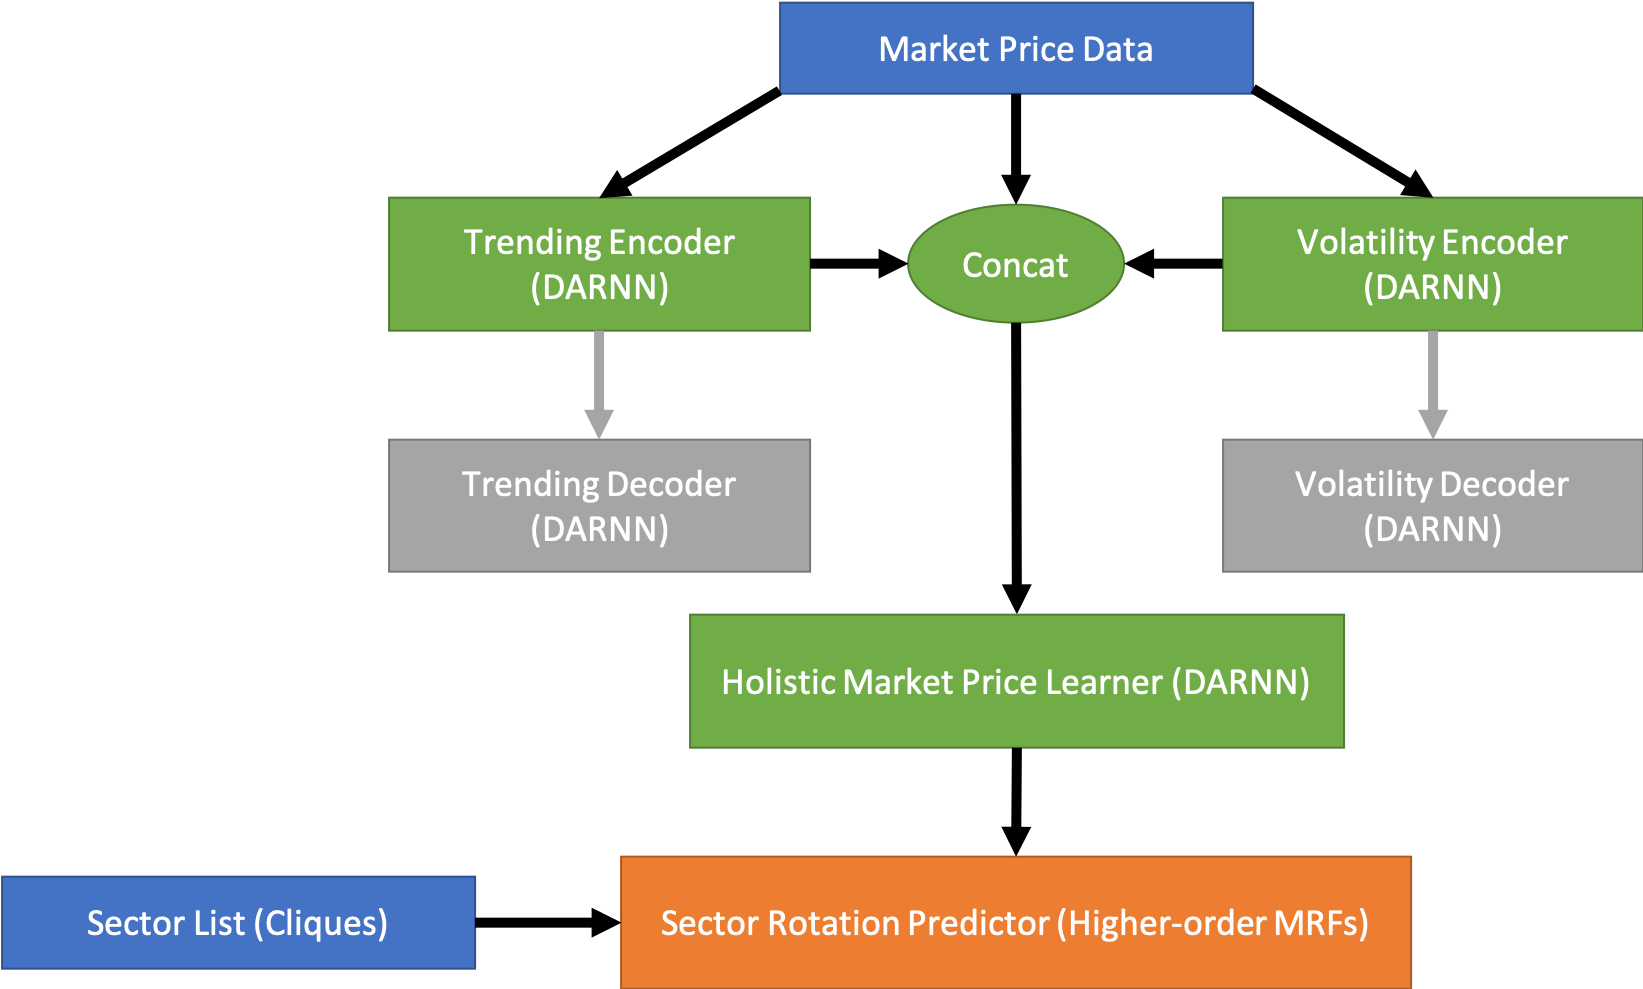
\includegraphics[width=1\columnwidth]{Methodology/figures/mrfrnn}
  \caption{\label{fig:mrfrnn} Multi-tasks DNN MRFs Architecture}
\end{figure}

All three DARNN modules share the same raw market price data.
Here we denote the time-series dataset as $\bX$ where
$\bX=(\bx_1,\bx_2,\dots,\bx_T)\in \reals^{N\times T}$. Here
$\bx^n=(x_1^n,x_2^n,\dots,x_T^n) \in \reals^T$ denotes a driving
series of $T$ time-steps and $\bx_t=(x_t^1,x_t^2\\ ,\dots
,x_t^N)\in \reals^N$ denotes a snapshot at time-step $t$ of all
$N$ driving series.

For both DARNN modules at the bottom level, the input matrix is a
concatenation of exogenous matrix $\bX \in \reals^{5\times T}$
which contains $5$ exogenous driving series: opening price, low
price, high price, volume, amount and $1$ target series $\by =
(y_1,y_2,\dots,y_T) \in \reals^T$. The task of those DARNNs are
to predict target series $y_{t+p}$ in the next $p$ time steps:

$$\hat{y}_{t+p} = \text{DARNN}(y_1,\dots,y_{t},x_1,\dots,x_t)$$

The target series $\by_{\text{trending}}$ of Trending DARNN is
closing price. The target series $\by_{\text{volatility}}$ of
Volatility DARNN is the standard deviation of closing price over
$T$ time-steps. We use Mean Squared Error (MSE) as loss function
to train those two modules separately.

To train the top level module, which is a classification DARNN,
we concatenate context vectors $\bc_t$ from each of bottom level
module's second stage encoder and raw market price matrix as
input matrix. The target series $\by^{\text{binary}}$ is
constructed by the sign function $y_t^{\text{binary}} =
sign(y_{t+p}-y_t)$ where $y_t$ denotes closing price at time-step
$t$. We use cross-entropy as loss function to train the final
DARNN. Logits (the output of the DARNN before going through the
softmax) of the final DARNN are passed to ``Sector Rotation
Predictor'' as unary features.

Since outputs of HMPL are only used as unary features in MRFs'
energy functions, our back-propagation rules can be defined by
taking derivative of equation~(\ref{eq:energyfunction_UPH}):

\begin{align}
  \label{eq:der_w}
  \frac{\partial L}{\partial \bw^U} = \phi^U(y)-\phi^U(y^*)
\end{align}

\noindent where $y$ is the ground-truth label and $y^*$ is
inferenced label. And

\begin{align}
  \label{eq:der_phi}
  \frac{\partial L}{\partial \phi^U} = \bw^U
\end{align}


\subsection{Sector Rotation Predictor}
\label{sec:srp}

We begin with a brief review of our choices of unary, pairwise
and higher-order potential functions. We then show how to perform
exact inference in models with these potentials. In
section~\ref{sec:learning} we will discuss learning the
parameters under the latent structural SVM framework and also how
to back-prop gradients to neural networks.


\subsubsection{Higer Order Energy: The Lower Linear Envelope Function}
\label{sec:llep}

From section~\ref{sec:MRF} we have already introduced that an
\emph{energy function} may contain \emph{unary}, \emph{pairwise}
and \emph{higher-order} potentials (see
equation~\eqref{eq:energyfunction_UPH}). In this section we
mainly focus on one class of higher-order potentials $\phi^H$
defined as a concave piecewise linear function which is known as
\emph{lower linear envelope potentials}. This has been studied
extensively in Markov Random Fields area for encouraging
consistency over large
cliques~\cite{Kohli:CVPR07,Nowozin:2011,Gould:ICML2011}.

Let $\C$ denotes the set of all maximal cliques in an image and
$\by_c=\{y_i |\text{\,for\,} i \in C_j\}$ denotes set of random
variables in the clique $C_j$, a weighted lower linear envelope
potential~\cite{gouldlearning} over $\by_c$ is defined as the
minimum over a set of $K$ linear functions as:
%
\begin{align}
  \psi^H_c\!(\by_c) \, &= \min_{k=1, \ldots, K} \left\{ a_k W_{\!c}(\by_c) + b_k \right\}.
  \label{eqn:potential2}
\end{align}
%
where $W_{\!c}(\by_c) = \sum_{i \in c} w_i y_i$ with $w^c_i \geq
0$ and $\sum_{i \in c} w^c_i = 1$ which are weights for each
clique. $(a_k, b_k) \in \reals^2$ are the linear function
parameters. We illustrate an example~\cite{gouldlearning} with
three linear functions in \figref{fig:nonredundant}.
% to_replace
\begin{figure}[ht]
  \centering
  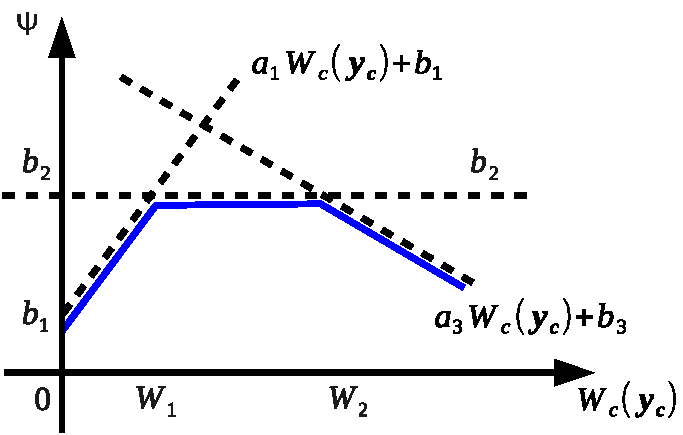
\includegraphics[width=0.6\columnwidth]{Methodology/figures/not_redundant}
  \caption{\label{fig:nonredundant} Example lower linear envelope
    $\psi^H_c\!(\by_c)$ (shown solid) with three terms (dashed).
    When $W_{\!c}(\by_c) \leq W_1$ the first linear function is
    active, when $W_1 < W_{\!c}(\by_c) \leq W_2$ the second
    linear function is active, otherwise the third linear
    function is active.}
\end{figure}

Inference on energy function contains lower linear potentials is
the same as the standard equation~\eqref{eq:energyfunction_UPH}
and is given by:
\begin{align}
  \label{eq:min_energy}
  \by^* = \argmin\energy{\by}
\end{align}

To ensure potentials do not contain redundant linear functions
(functions that would never be active), \citename{gouldlearning}
proposed a constraint on parameters of the envelope. The $k$-th
linear function is not redundant if the following condition is
satisfied:
%
\begin{align}
    0
    <
    \frac{b_k - b_{k-1}}{a_{k-1} - a_k}
    <
    \frac{b_{k+1} - b_k}{a_k - a_{k+1}}
    <
    1.
  \label{eq:nonredundant}
\end{align}
%
Another important property of equation~\eqref{eq:min_energy} is
shift invariant~\cite{gouldlearning} (vertically). We write
$\widetilde{\psi}^{H}_c\!(\by_c)$ by shift equation~\eqref{eqn:potential2} vertically
with an abitrary amount $b^{const}\in R$
$$\widetilde{\psi}^{H}_c\!(\by_c) = \min_{k=1, \ldots, K}
\left\{a_k W_{\!c}(\by_c) + b_k + b^\textrm{const} \right\}$$
%
Then we have
\begin{align}
  \argmin_{\by_c} \psi^H_c\!(\by_c)
  = \argmin_{\by_c} \widetilde{\psi}^{H}_c\!(\by_c).
  \label{eq:shift_invariant}
\end{align}
%
Therefore, in the following discussion without loss of generality
we assume $b_1 = 0$ thus $b_k\geq0 \text{\; for \;} k=1,\dots,n$.
%
\subsubsection{Exact Inference}
\label{sec:exact_inference}

Exact inference on MRFs has been extensively studied in past
years. Researchers found that, energy functions which can be
transformed into quadratic pseudo-Boolean
functions~\cite{Ishikawa:PAMI03,Ishikawa:CVPR09,Rother:CVPR09}
are able to be minimized exactly using \emph{graph-cuts} like
algorithms~\cite{Freedman:CVPR05,Hammer:1965} when they satisfy
submodularity condition~\cite{Boros:MATH02}.
\citename{Kohli:TR08} and \citename{Gould:ICML2011} adapted those
results to perform exact inference on lower linear envelope
potentials. In this section we mainly focus on describing the
\emph{st min cut} graph constructed by
Gould~\cite{Gould:ICML2011,gouldlearning} for exact
inference~\eqref{eq:min_energy} of energy function containing
lower linear envelope potentials.

Following the approach of \citename{Kohli:CVPR10},
\citename{Gould:ICML2011,gouldlearning} transformed the weighted
lower linear envelope potential~\eqref{eqn:potential2} into a
quadratic pseudo-Boolean function by introducing $K-1$ auxiliary
variables $\bz = \left(z_1, \ldots, z_{K-1}\right)$ with $z_k\in
\{0,1\}$:

\begin{align}
  E^c(\by_c, \bz) &= a_1 W_{\!c}(\by_c) + b_1 \notag \\
  &+ \sum_{k = 1}^{K-1} z_k \left( \left(a_{k+1} - a_k\right) W_{\!c}(\by_c) + b_{k+1} - b_k \right)
  \label{eqn:binary_concave_z}
\end{align}

\noindent for a single clique $c \in \C$. Under this formulation,
minimizing the pseudo-Boolean function over $\bz$ is equivalent
to selecting (one of) the active functions(s) from
equation~\eqref{eqn:potential2}. Another important property of
optimized $\bz$ under this formulation is that it automatically
satisfies the constraint~\cite{gouldlearning}:

\begin{figure}[t]
  \centering
  \setlength{\tabcolsep}{2pt}
  \begin{tabular}{cc}
    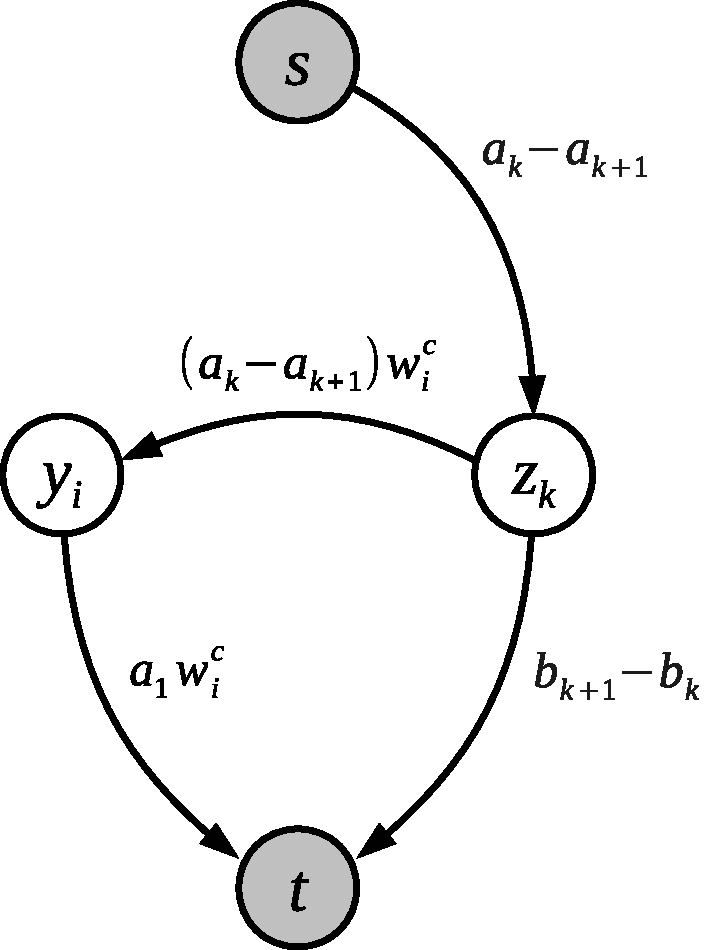
\includegraphics[width=0.45\columnwidth]{Methodology/figures/stmincut}&
                                                                         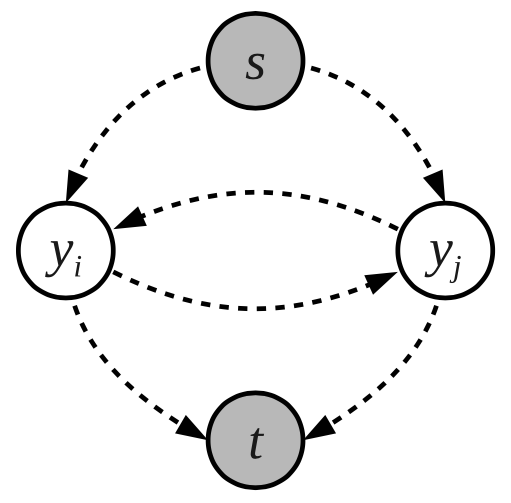
\includegraphics[width=0.5\columnwidth]{Methodology/figures/unary_pairwise.png}\\
                                                                         {\small (a)} & {\small (b)} 
  \end{tabular}
  \caption{\label{fig:stmincut} $st$-graph
    construction~\cite{gouldlearning} for
    equation~\eqref{eqn:posiform}, unary and pairwise terms.
    Every cut corresponds to an assignment to the random
    variables, where variables associated with nodes in the
    ${\cal S}$ set take the value one, and those associated with
    nodes in the $\T$ set take the value zero. With slight abuse
    of notation, we use the variables to denote nodes in our
    graph.}
\end{figure}

\begin{align}
  \label{eq:z_consecutive_constraint}
  z_{k+1} \leq z_k
\end{align}

\noindent this property give rise to further development of
parameter vector~\eqref{eq:llsvm_param} and feature
vector~\eqref{eq:llsvm_feature} which are used in latent
structural SVM.

In order to construct the \emph{st-min-cut} graph, we rewrote
equation~\eqref{eqn:binary_concave_z} into
\emph{posiform}~\cite{Boros:MATH02}:

\begin{align}
  \label{eqn:posiform}  
  E^c(\by_c, \bz)
  &= b_1 - (a_1 - a_K) + \sum_{i \in c} a_1 w^c_i y_i \notag\\
  & + \sum_{k = 1}^{K - 1} \left( b_{k+1} - b_k \right) z_k
    + \sum_{k = 1}^{K - 1} \left( a_k - a_{k+1} \right)
    \bar{z}_k\notag\\
  & + \sum_{k = 1}^{K - 1} \sum_{i \in c} \left( a_k - a_{k+1}
    \right) w^c_i \bar{y}_i z_k
\end{align}

\noindent where $\bar{z}_k = 1 - z_k$ and $\bar{y}_i = 1 - y_i$.
$a_1$ is assumed to be greater than $0$ so that all coefficients
are positive (recall we assume $b_1=0$ in section~\ref{sec:llep}
and we have $a_k > a_{k+1}$ and $b_k < b_{k+1}$). After proving
\emph{submodularity} of the energy function~\eqref{eqn:posiform},
\citename{gouldlearning} constructed the \emph{st-min-cut} graph
based on equation~\eqref{eqn:posiform}.

The construction is explained in \figref{fig:stmincut}. Figure
(a) denotes construction for equation~\eqref{eqn:posiform}. For
each lower linear envelope potential edges are added as follows:
for each $i \in c$, add an edge from $y_i$ to $t$ with weight
$a_1 w^c_i$; for each $i \in c$ and $k = 1, \ldots, K-1$, add an
edge from $z_k$ to $y_i$ with weight $(a_{k} - a_{k+1}) w^c_i$;
and for $k = 1, \ldots, K-1$, add an edge from $s$ to $z_k$ with
weight $a_k - a_{k+1}$ and edge from $z_k$ to $t$ with weight
$b_{k+1} - b_k$. Figure (b) denotes construction for unary and
pairwise terms (see \cite{Kolmogorov:PAMI04}). For unary edges (4
edges on both sides), weights on each edge are corresponding to
values in input unary terms accordingly. For pairwise edges (2
edges in the middle), both edges share the same weight which
equals to the input pairwise term.
% todo: unary from RNN

\section{Optimization}
\label{sec:opt}

% todo: experiment no pairwise features

\subsection{Transforming Between Representations}
\label{sec:learning}
With the inference algorithm in hand, we now can develop the
learning algorithm for weighted lower linear envelope potentials
using the latent structural SVM framework. We begin by
transforming the equation~\eqref{eqn:binary_concave_z} into a
linear combination of parameter vector and feature vector. Then a
two-step algorithm was developed to solve the latent structural
SVM.

The latent structural SVM formulation (see
equation~\eqref{eq:latent_ssvm_linearcomb}) requires that the
energy function be expressed as a linear combination of features
and weights while our higher-order potential is represented as
the minimum over a set of linear functions. However,
in~\ref{sec:exact_inference} we reformulated the piesewise linear
functions into a quadratic pseudo-Boolean
function~\eqref{eqn:binary_concave_z} by introducing auxiliary
variables. Now we show function~\eqref{eqn:binary_concave_z}
itself is an inner product of parameter vector and feature vector
with latent information. We first noticed that the function can
be expanded as a summation of $2K-1$ terms:

\begin{align}
  \label{eq:originalenergy}
  E^c(y_c,z)=&a_1W_c(y_c)+b_1\notag \\
            &+\sum_{k=1}^{K-1}z_k((a_{k+1}-a_k)W_c(y_c)+b_{k+1}-b_k)\notag \\ 
            =&a_1W_c(y_c)+\sum_{k=1}^{K-1}(a_{k+1}-a_k)z_kW_c(y_c) \notag \\
            &+\sum_{k=1}^{K-1}(b_{k+1}-b_k)z_k
\end{align}

Here we use the fact of equation~\eqref{eq:shift_invariant} and
let $b_1=0$. Now we can reparameterize the energy function
as
\begin{align}
  \label{eq:llsvm_innerprod_energy}
  E^c(\by_c,\bz; \btheta) = \btheta^T \! \phi(\by_c,\bz)
\end{align}

\noindent where:

\begin{equation}
\label{eq:llsvm_param}
  \theta_k = \left\{
    \begin{aligned}
      & a_1	& \text{for} \ k=1\\
      & a_k-a_{k-1} & \text{for}\ 1< k \leq K\\
      & b_{k+1-K}-b_{k-K} & \text{for} \ K<k\le2K-1\\
    \end{aligned}
  \right.
\end{equation}

\begin{equation}
\label{eq:llsvm_feature}
  \phi_k = \left\{
		\begin{aligned}
      & W_c(\by_c) 	& \text{for} \ k=1\\
      & W_c(\by_c)\bz_k & \text{for}\ 1<k\le K\\
      & \bz_k & \text{for} \ K<k\le2K-1\\
		\end{aligned}
  \right.
\end{equation}

Under this formulation, inference
problems~\eqref{eq:latentssvm_full_inf}
and~\eqref{eq:latentssvm_latent_inf} introduced in
section~\ref{sec:latent-struct-svms} can be written as:

\begin{align}
  \label{eq:linenv_full_inf}
  (\mathbf{\hat{y}}_k(\btheta),\mathbf{\hat{z}}_k(\theta))=\argmin_{(\mathbf{y}
  \times \mathbf{z}) \in \mathcal{Y} \times \mathcal{Z}}
  \btheta^T\cdot\phi(\mathbf{y}_k,\mathbf{z}_k)
\end{align}
and
\begin{align}
  \label{eq:linenv_latent_inf}
  \mathbf{z}^*_k(\btheta) = \argmin_{\mathbf{z} \in \mathcal{Z}}
  \btheta^T \cdot \phi(\mathbf{y}_k,\mathbf{z}_k)
\end{align}

There are 2 facts worth to mention. The first fact is
that in our previous construction of minimum-$st$-cut graph the
latent variable $\bz$ is already included. Therefore, we can
apply our inference algorithm directly on our 2 new formulations.

However, for equation~\eqref{eq:linenv_latent_inf} there exists
more efficient algorithm. At training stage the ground-truth
labels $y_i$ is a function input thus completely observed.
Therefore, the term $((a_{k+1}-a_k)W_c(\by_c)+b_{k+1}-b_k)$ in
equation~\eqref{eq:originalenergy} becomes constant. So we can
infer latent variable $\bz$ explicitly by:
\begin{align}
  \label{eq:linenv_effi_infer_latent}
  z_k^c &=
          \begin{cases}
            0 & \text{if $((a_{k+1}-a_k)W_c(y_c)+b_{k+1}-b_k)\geq0$} \\
            1 & \text{otherwise}.
          \end{cases}
\end{align}

\begin{figure}[t]
  \centering
  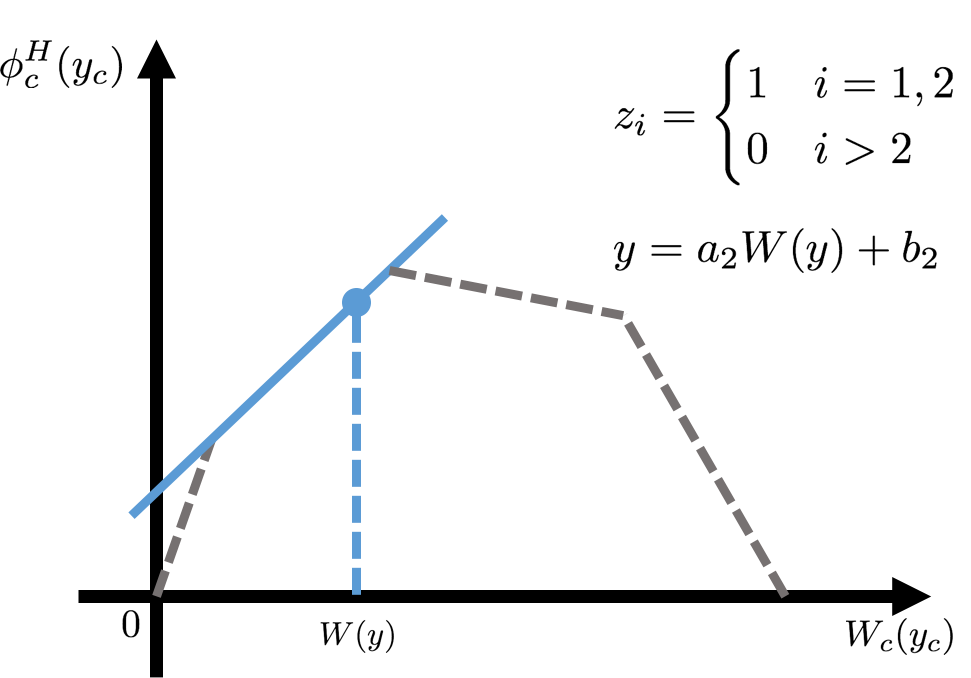
\includegraphics[width=0.8\columnwidth]{Methodology/figures/linEnvLatentFig.png}
  \caption{\label{fig:concave} Example piecewise-linear concave
    function of $W_{\!c}(\by_c) = \sum_{i \in c} w^c_i y_i$.
    Assume the second linear function is active namely
    $\bz^c=(1,1,0,0)$. The result of linear combination of
    parameter vector and feature vector is same as quadratic
    psuedo-Boolean function.}
\end{figure}

Therefore, assignments inferred by graph-cut algorithm can be
directly encoded into a linear combination by using our latent
structural SVM formulation for learning purpose. The remaining
task is to ensure the concavity of $\btheta$. We do this by
adding the following constraint:

\begin{align}
  A\btheta\geq0 \text{,\;~~~} A=
                  \begin{bmatrix}
                    1 & \mathbf{0} & \mathbf{0}\\
                    \mathbf{0} & -\mathbf{1} & \mathbf{0}\\
                    \mathbf{0} & \mathbf{0} & \mathbf{P}
                  \end{bmatrix}\in \mathbb{R}^{(2K-1)\times(2K-1)}
\end{align}

\noindent where $-\mathbf{1}$ is a matrix of size $(K-1)\times(K-1)$ and
$\mathbf{P}$ is an identity matrix of size $(K-1)\times(K-1)$.

One subtle problem we found during experiments is that the
algorithm can be stuck with small numerical value. To avoid this
we add small slack variables $\epsilon$ on those constraints:

\begin{align}
  \label{eq:concave_constraint}
  A\btheta\geq\epsilon \text{,\;~~~} A=
                  \begin{bmatrix}
                    1 & \mathbf{0} & \mathbf{0}\\
                    \mathbf{0} & -\mathbf{1} & \mathbf{0}\\
                    \mathbf{0} & \mathbf{0} & \mathbf{P}
                  \end{bmatrix}\in \mathbb{R}^{(2K-1)\times(2K-1)}
\end{align}

\noindent where $\epsilon$ equals to $\mathbf{1}^{-15}$ in our
experiments.

\subsection{Latent Structural SVM Learning}
\label{sec:mrflssvm_learning_algo}

With the inner product formulation
(equation~\eqref{eq:llsvm_innerprod_energy}) of higher order
energy function in hand, we now able to develop our latent
structural SVM learning algorithm. The energy function (higher
order function together with unary and pairwise functions) can be
written as:
\begin{equation}
  E_{all}(y,z) = \begin{bmatrix}
    \btheta^H\\
    \theta^{unary}\\
    \theta^{pairwise}
  \end{bmatrix}^T 
  \cdot \begin{bmatrix}
    \phi^H\\
    \phi^{unary}\\
    \phi^{pairwise}
  \end{bmatrix}=\theta_{all}^T\cdot\phi_{all}
\end{equation}
where $\btheta^H\in \reals$ is the parameter vector in higher
order equation~\eqref{eq:llsvm_innerprod_energy} of size $2K-1$.
$\theta^{unary}$ and $\theta^{pairwise}$ are both scalars.
$\phi^\textrm{unary} = \sum_i \psi^U_i\!(y_i)$ and
$\phi^\textrm{pairwise} = \sum_{ij} \psi^P_{ij}(y_i, y_j)$.
Therefore, the size of $\theta_{all}$ is $2K+1$.

Plug equation~\eqref{eq:linenv_full_inf} and
equation~\eqref{eq:linenv_latent_inf} into object
function~\eqref{eq:latent_ssvm_object}, the latent structural SVM
object function for our problem can be derived as a difference of
two convex functions:

\begin{align}
\label{eq:lssvm_object}
  \min_\theta\bigg(\frac{1}{2}\|\theta\|^2+
  C\sum_{i=1}^{n}\big(\max_{(\mathbf{\hat{y}} \times
  \mathbf{\hat{z}}) \in \mathcal{Y} \times \mathcal{Z}}
  [\theta\cdot\phi(\mathbf{\hat{y}},\mathbf{\hat{z}}) +
  \Delta(\mathbf{y}_i,\mathbf{\hat{y}},\mathbf{\hat{z}})]\big)\bigg)\\
  -C\sum_{i=1}^{n}\big(\max_{\mathbf{z} \in \mathcal{Z}} \theta \cdot
  \phi(\mathbf{y}_i,\mathbf{z})\big)\nonumber
\end{align}

As mentioned by \citename{yu2009learning} the Concave-Convex
Procedure (CCCP)~\cite{yuille2002concave} can be used to solve the
optimization problem. Our algorithm contains two stages. We first
imputes the latent variables $\bz$ explicitly by
equation~\eqref{eq:linenv_latent_inf}. Namely solving the
``latent variable completion'' problem~\cite{yu2009learning}:

\begin{align}
  \bz_i^*=\argmax_{\mathbf{z} \in \mathcal{Z}} \theta \cdot
  \phi(\mathbf{y}_i,\mathbf{z})
\end{align}

The inference result $z_i^*$ for $i=1,\dots,n$ is used as
completely observed for later stage. With the latent variable
$z_i^*$ which best explains the ground-truth data $y_i$ in hand,
updating the parameter vector $\btheta$ is similar to solve the
standard max-margin optimization problem described
in~\cite{gouldlearning}:

\begin{align}
\label{eq:mrflssvm_object}
  \min_\theta\bigg(\frac{1}{2}\|\theta\|^2+
  C\sum_{i=1}^{n}\big(\max_{(\mathbf{\hat{y}} \times
  \mathbf{\hat{z}}) \in \mathcal{Y} \times \mathcal{Z}}
  [\theta\cdot\phi(\mathbf{\hat{y}},\mathbf{\hat{z}}) +
  \Delta(\mathbf{y}_i,\mathbf{\hat{y}},\mathbf{\hat{z}})]\big)\bigg)\\
  -C\sum_{i=1}^{n}\big(\theta \cdot
  \phi(\mathbf{y}_i,\mathbf{z}_i^*)\big) \nonumber
\end{align}

The last problem remaining is the initialization method. Because
our objective function~\eqref{eq:mrflssvm_object} is not convex
and the CCCP algorithm is only guaranteed to converge to a local
minimum or saddle point\cite{yuille2002concave}, initialization
of $\btheta$ might affect the performance of our algorithm. Since
there are no theoretical solution for this problem, we only
propose an empirical \algref{alg:init_theta}:

\begin{algorithm}[ht]
  \begin{algorithmic}[1]
    \STATE{$gap=\frac{1}{K}$, $a_1=\U(0,1e6)$, $b_1=0$,
      $sp_1=(0,0)$, $w_0=0$, $counter=2$} \FOR{each
      clique $c\in \C$} \STATE{Compute weighted clique value
      $w_c=W_c(y_C)$} \IF{$w_c-w_{c-1}>gap$}
    \STATE{$upbound = a_{counter}w_c+b_{counter}$\\
      $sp_{counter}=(w_c,\U(upbound-0.5,upbound))$\\
      Calculate $a_{counter}$ and $b_{counter}$ using
      $sp_{counter-1}$ and $sp_{counter}$\\
      $counter=counter+1$}
    \ENDIF
    \ENDFOR
    \STATE{If $counter<K$, remaining $a$s and $b$s are all set to
      be $a_{counter}$ and $b_{counter}$} \STATE{Calculate
      $\btheta$ using $\{a_k,b_k\}_{k=1}^K$}
  \end{algorithmic}
  \caption{\label{alg:init_theta} Empirical initialization
    algorithm for $\btheta$}
\end{algorithm}

We assume that the more evenly distributed of $W_c(Y_c)$ where
$c\in\C$ on $x$ axis, the more rich representation (number of
linear functions) the energy function should have. In order to
initialize $\btheta$, we first determine the x-coordinate of
sampled points $sp$. Then we sample its y-coordinate from a
uniform distribution $\U(upbound,upbound-0.5)$ to add some
randomness in our initialization as well as maintain concavity.
Linear parameters $a_k$ and $b_k$ are later calculated using
those sampled points $sp_k$ and $sp_{k-1}$. At last we encode
$\{a_k,b_k\}_{k=1}^K$ into $\btheta$ using
equation~\eqref{eq:llsvm_param}.

Our optimization algorithm is summarized in
\algref{alg:learning}.

\begin{algorithm}[hb]
  \begin{algorithmic}[1]
    \STATE{Set $MaxIter = 100$}
    \STATE{ {\bf input} training set $\{\by_i\}_{i=1}^{n}$, regularization constant $C > 0$,
      and tolerance $\epsilon \geq 0$}
    \STATE{Initialize $\btheta$ using \algref{alg:init_theta}}
    \REPEAT
    \STATE{Set $iter = 0$}
    \FOR{each training example, $i = 1, \ldots, n$}
    \STATE{compute $ \bz_i^*=\argmax_{\mathbf{z} \in \mathcal{Z}}
      \theta \cdot \phi(\mathbf{y}_i,\mathbf{z}) $}
    \ENDFOR

    \STATE{ {\bf initialize} active constraints set $\C_i = \{ \}$ for all $i$}
    \REPEAT

    \STATE{solve the quadratic programming problem in
      equation~\ref{eq:mrflssvm_object} with respect to active
      constraints set $\C_i$ for all $i$ and concavity constraints
      $A\btheta\geq \epsilon$ to get
      $\hat{\btheta}$ and $\hat{\bxi}$}

    \FOR{each training example, $i = 1, \ldots, n$}
    \STATE{compute $\hat{\by_i},\hat{\bz_i} = \argmin_{\by}
      E(\by,\bz; \hat{\btheta}) - \Delta(\by, \bz, \by_i)$}
    \IF{$\hat{\xi}_i + \epsilon \!<\! \Delta(\hat{\by_i},
      \hat{\bz_i}, \by_i) -
      E(\hat{\by_i},\hat{\bz_i}; \hat{\btheta}) + E(\by_i, \bz_i^*; \hat{\btheta})$}
    \STATE{$\C_i \leftarrow \C_i \cup \{\by_i^\star\}$}
    \ENDIF
    \ENDFOR
    \UNTIL{no more violated constraints}
    \STATE{ {\bf return} parameters $\hat{\btheta}$}
    \STATE{Set $iter = iter+1$}

    \UNTIL{$iter\geq MaxIter$}
    \STATE{ {\bf return} parameters $\hat{\btheta}$}
  \end{algorithmic}
  \caption{\label{alg:learning} Learning lower linear envelope
    MRFs with latent variables.}
\end{algorithm}


\section{Experiment}
\label{sec:exp}

\subsection{Dataset}
\label{sec:dataset}

Momentum: Awesome Oscillator, Money Flow Index
Volume: Chaikin Money Flow, On-balance volume mean
Volatility: Bollinger Bands (Upper and Lower Bands)
Trend: Average Directional Movement Index, Moving Average Convergence Divergence

240 a day,
validation test dataset 5 million
train dataset 40 million 2015-01-05 to 2017-05-31


\newcommand{\newblock}{}
\setcitestyle{numbers} % set the citation style to ``numbers''.
\bibliographystyle{plainnat}
\bibliography{Bibs/thesis,Bibs/long,Bibs/scene,Bibs/proposal,Bibs/fin}

% That's all folks!
\end{document}
